\documentclass[sigconf]{acmart}

\usepackage{booktabs}

\settopmatter{printacmref=false}

\renewcommand\footnotetextcopyrightpermission[1]{}

\pagestyle{plain}

\begin{document}
\title{SET10107 Computational Intelligence Coursework}
\acmConference[SET10107]{Coursework}{April 2018}{Edinburgh Napier University} 
\acmYear{2018}
\copyrightyear{2018}

\author{Beej Persson, 40183743@live.napier.ac.uk\\School of Computing, Edinburgh Napier University, Edinburgh}



\begin{abstract}
An investigation into the performance of evolutionary algorithm via the introduction of varied operators and a manipulation and exploration of the neural network's parameters.
\end{abstract}



\keywords{evolutionary algorithm, neural network}


\maketitle

\section{Approach}

\subsection{Background}
There are some problems that are often unsolvable in a reasonable time frame if an exact solution is desired. Evolutionary Algorithms provide a way to solve these problems within a reasonable time limit and can produce solutions that may not be exact but good enough. 

An Evolutionary Algorithm are ``search algorithms gleaned from organic evolution'' \cite{back96}. They are built with the intention to provide a reasonable solution by encouraging the creation of children produced from strong individuals. The children can then be slightly mutated before being put back into the population. In this way a form of evolution occurs.

For the purposes of this project an evolutionary algorithm was used to evolve a neural network than controls the landing of numerous spacecraft that are spawned somewhere above the the landing zone. The desire is to produce a solution that can land as many spacecraft as possible by manipulating the parameters and operators of the algorithm.

\subsection{Evolutionary Algorithm}
The evolutionary algorithm used in this project was based off an algorithm provided as part of the coursework. First, a population of individuals is initialised with random weights that affect the outputs, which control the spacecraft's thrusters. Two parents are selected from the population of individuals and, via reproduction, from them two children created. At this stage the child individuals are mutated in an attempt to bring about improvements. Their fitness is then evaluated, defined as a function of their distance from the landing zone, their relative velocity on landing and their thruster fuel remaining. They are then placed into the population via a process of replacing an existing member. The individual with the best fitness has their fitness printed out and the process repeats from the selection stage for a set number of times. After all the desired evolutions have been carried out, the individual with the best fitness in the population is saved to a file.

\subsection{Operators}
A number of key operators exist in the evolutionary algorithm, the details of their role are described below:
\subsubsection{Selection}
To select the two parents, a tournament with a subset of the population is held. The number of individuals in the tournament can be changed as a parameter. The tournament list is created using random individuals from the population and the individual with the lowest fitness is chosen. There are other ways selection can happen, for example a random member of the population can be chosen and used to produce children or the individual with the lowest fitness can be chosen. However this can increase the selection pressure and cause premature convergence. The reason for not exploring other selection methods is based on the research that was done, and a tournament selection method was shown to be appropriate for needs of this problem \cite{blickle96} \cite{goldberg91}.
\subsubsection{Reproduction}
To reproduce the two parents a number of algorithms were implemented and tested. The best performers were the Uniform Crossover and n-Point Crossover algorithms. 1-Point Crossover and Arithmetic Crossover was also implemented and all underperformed in comparison to Uniform. In Uniform, each gene in the child chromosomes are made by choosing random genes from each parent. 1-Point selects a random point along each parent chromosome, and gives one half of the genes to one child and the other half to the other child. For n-Point this process is repeated but for a larger number of cut points. If the number of points is equal to the number of genes, then n-Point Crossover is effectively identical to Uniform Crossover. The final reproduction method was Arithmetic Crossover. This is where the arithmetic average of the two values in each of the corresponding genes of the parents is given to the children.
\subsubsection{Replacement}
Three approaches to replacement were considered, with two performing very similarly. The first method was to replace the worst two individuals in the population with the newly created children. This would regularly cause premature convergence in a similar way that can happen when selecting the best parent. Another replacement method that performed inconsistently was random replacement. By replacing random members of the population, sometimes the fittest would be removed and other times the worst. There was also a tournament replacement method implemented that worked similarly to the selection tournament, except for finding the worst individual. With appropriate tournament sizes to reduce replacement pressure, this was found to work well.

\subsection{Parameters}
Further to the operators that were implemented and tested, a number of the neural network's parameters were changed in attempts to produce better results. The details of these parameters are described below:
\subsubsection{Hidden Nodes}
Hidden Nodes are the nodes that appear in the Hidden Layer of the algorithm. This layer is between the input layer and the output layer and is how the weights of the chromosomes are passed as outputs. The number of nodes in the Hidden Layer affects the number of weights in the chromosome, increasing their number can cause overfitting the solution, and reducing them can cause underfitting \cite{panchal11}.
\subsubsection{Population}
The population parameter simply allows the adjustment of the size of the initial population created.
\subsubsection{Mutation}
There are two mutation parameters, \textit{mutateRate} and \textit{mutateChange}. The rate affects how often a child is muted before being inserted into the population, and the change affects how much it is mutated by.
\subsubsection{Tournament Size}
The tournament size parameters were two new parameters created to allow the size of the tournament list used in the selection and replacement algorithms to be changed.
\subsubsection{Max Evaluations}
The max evaluations parameter controlled the number of maximum evaluations of the evolutionary algorithm before the process would stop. This was set to 20,000 evaluations and was not changed for the duration of the testing. 

\section{Experiments and Analysis}
\subsection{Operators Exploration}
Initially an exploration of the performance of the algorithm with its base operators was undertaken. As a number of operator methods had been introduced, these needed to be tested too and the optimal combination found. For the purposes of these tests all the neural network parameters were left at their default setting, shown in Table \ref{defparamstable}.

\begin{table}[!h]
	\renewcommand{\arraystretch}{1.3}
	\caption{Default Parameters}
	\label{defparamstable}
	\begin{tabular}{l|c}
		\toprule
		\textbf{Parameter} & \textbf{Value} \\ \midrule
		Hidden Nodes & 5\\ \hline
		Population Size & 200 \\ \hline
		Mutation Rate & 0.01\\ \hline
		Mutation Change & 0.05\\ \hline
		Tournament Sizes & 20 \\ \hline
		Max Evaluations & 20,000 \\ \bottomrule
	\end{tabular}
\end{table}

All testing carried out in this project consisted of running a loop of 20,000 evaluations on a training dataset, and then determining the best individual's fitness on the training dataset and finding its fitness when ran on a test dataset. Each loop was tested 10 times and the average fitness performance recorded. The results of the tests on the added operators is shown in Tables \ref{reproductiontable} and \ref{replacementtable}:

\begin{table}[!h]
	\caption{Reproduction Operator Method Comparison}
	\label{reproductiontable}
	\centering
	\resizebox{\columnwidth}{!}{%
		\begin{tabular}{c|cc}
			\toprule
			Reproduction Method & Training Fitness & Test Fitness \\ \midrule
			Uniform & 0.113220349 & 0.232088989 \\
			1-Point & 0.126216203 & 0.266498011 \\
			nPoint & 0.11239654 & 0.243947017 \\ 
			Arithmetic & 0.134360733 & 0.266206789 \\ \bottomrule
		\end{tabular}%
	}
\end{table}

\begin{table}[!h]
	\caption{Replacement Operator Method Comparison}
	\label{replacementtable}
	\centering
	\resizebox{\columnwidth}{!}{%
		\begin{tabular}{c|cc}
			\toprule
			Replacement Method & Training Fitness & Test Fitness \\ \midrule
			Tournament & 0.107673501 & 0.233794064 \\
			Random & 0.123415836 & 0.250230224 \\
			Worst & 0.126216203 & 0.266498011 \\ \bottomrule
		\end{tabular}%
	}
\end{table}

Another test was done solely on the nPoint Crossover's performance, the results of which are not shown, where it was found that increasing the number of cut points did not seem to affect the average fitness results.

From the findings, it was clear that the results were all fairly close. Uniform and nPoint Crossover slightly outperformed 1-Point and Arithmetic Crossover. Tournament replacement produced lower average fitness than both Random replacement and Worst replacement.

\subsection{Parameter Tuning}
From here a thorough parameter tuning and evaluation was conducted using the same testing process described earlier. Due to the operator testing results, Uniform Crossover and Tournament Replacement were used throughout the parameter testing. Tournament Selection was used based on the research discussed earlier.

\subsubsection{Hidden Nodes}
The first parameter manipulated was the number of Hidden Nodes. The average fitness results on both the training dataset and the test dataset are shown below in Table \ref{nodetable}.

\begin{table}[!h]
	\caption{Number of Hidden Nodes Comparison}
	\label{nodetable}
	\centering
	\resizebox{\columnwidth}{!}{%
		\begin{tabular}{c|cc}
			\toprule
			Nodes & Training Fitness & Test Fitness \\ \midrule
			2 & 0.131139376 & 0.269929663 \\
			3 & 0.109574187 & 0.220307361 \\
			4 & 0.117917921 & 0.253313491 \\
			5 & 0.112005125 & 0.237632857 \\
			6 & 0.124126673 & 0.254198127 \\
			7 & 0.107124734 & 0.233553677 \\
			10 & 0.118745749 & 0.26061414 \\ \bottomrule
		\end{tabular}%
	}
\end{table}

From these results it was concluded that the number of Hidden Nodes rarely had much affect on the performance of my evolutionary algorithm.

\subsubsection{Population}
After this the size of the population was varied from $50$ to $450$. The average fitness results of both the training and test datasets can be seen in Table \ref{poptable}.

\begin{table}[!h]
	\caption{Size of Initial Population Comparison}
	\label{poptable}
	\centering
	\resizebox{\columnwidth}{!}{%
		\begin{tabular}{c|cc}
			\toprule
			Population Size & Training Fitness & Test Fitness \\ \midrule
			50 & 0.13753437 & 0.259774397 \\
			100 & 0.133925738 & 0.264025819 \\
			150 & 0.116352982 & 0.256550953 \\
			200 & 0.124908912 & 0.263566696 \\
			250 & 0.119553628 & 0.263334386 \\
			300 & 0.118354139 & 0.257590852 \\
			350 & 0.107322415 & 0.206113286 \\
			400 & 0.114187707 & 0.240516193 \\
			450 & 0.111521678 & 0.246246767 \\ \bottomrule
		\end{tabular}%
	}
\end{table}

One again it seemed to have no noticeable affect on the average fitness of the best individual produced.

\subsubsection{Mutation}
The first real changes came about with the mutation changes. Whilst changing the amount that it would mutate by manipulating the \textit{mutateChange} parameter seemed to produce similar results to before (shown in Table \ref{mutchangetable}), changing the mutation rate showed some slight improvements.

\begin{table}[!h]
	\caption{Mutate Change Parameter Comparison}
	\label{mutchangetable}
	\centering
	\resizebox{\columnwidth}{!}{%
		\begin{tabular}{c|cc}
			\toprule
			Mutate Change & Training Fitness & Test Fitness \\ \midrule
			0.05 & 0.114435572 & 0.226545121 \\
			0.1 & 0.111650377 & 0.24051258 \\
			0.15 & 0.115642614 & 0.250906451 \\
			0.2 & 0.105309223 & 0.2313873 \\ \bottomrule
		\end{tabular}%
	}
\end{table}

As can be seen in Table \ref{mutratetable} and Figure \ref{mutategraph} changing the mutation rate produced the lowest results for fitness yet. The graph showed that with a mutation rate of around 15\%, the results for average fitness on the training dataset were as low as $0.079$, a significant improvement.

\begin{table}[!h]
	\caption{Mutation Rate Parameter Comparison}
	\label{mutratetable}
	\centering
	\resizebox{\columnwidth}{!}{%
		\begin{tabular}{c|cc}
			\toprule
			Mutate Rate & Training Fitness & Test Fitness \\ \midrule
			0.01 & 0.114435572 & 0.226545121 \\
			0.03 & 0.110551575 & 0.237138597 \\
			0.05 & 0.1076695 & 0.24183747 \\
			0.1 & 0.109895118 & 0.254196016 \\
			0.15 & 0.079046816 & 0.206449561 \\
			0.2 & 0.113587067 & 0.249484968 \\ \bottomrule
		\end{tabular}%
	}
\end{table}

\begin{figure}[!h]
	\centering
	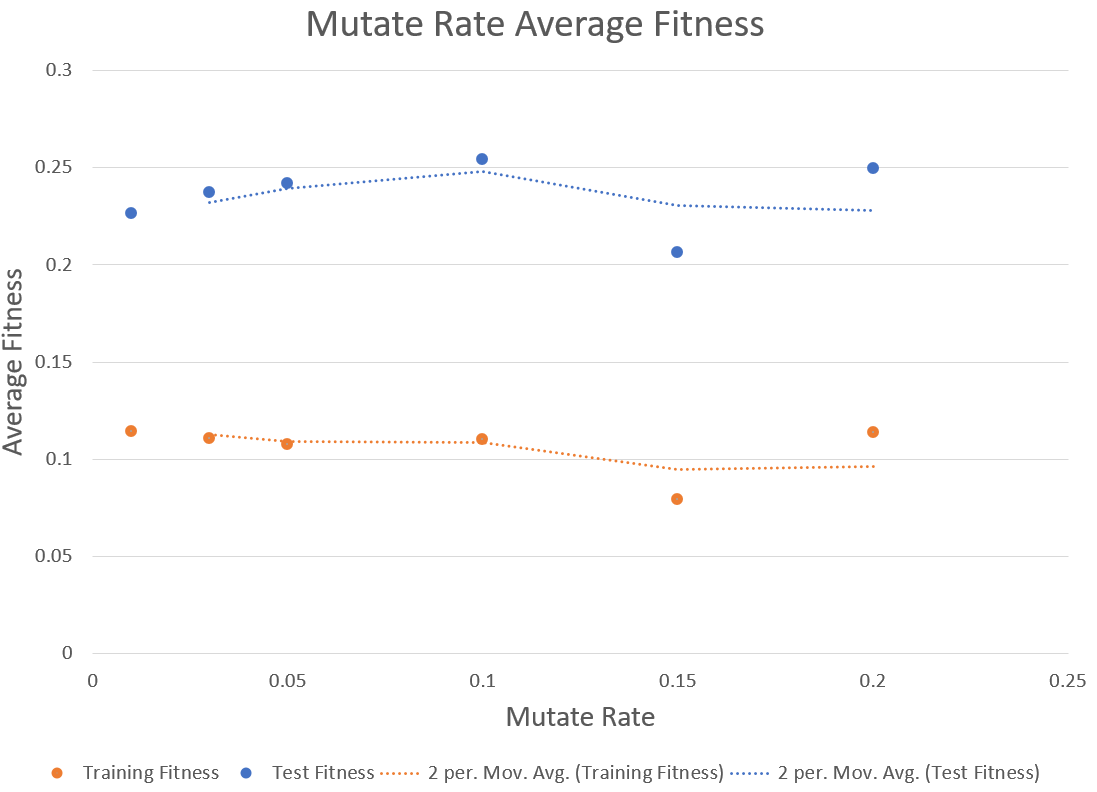
\includegraphics[width=\columnwidth]{IMAGES/mutaterate}
	\caption{Mutation Rate Fitness Averages.}
	\label{mutategraph}
\end{figure}

\subsubsection{Tournament Sizes}
The final parameter adjusted was the tournament sizes for both the selection and replacement method. The results for average fitness when changing the tournament for the selection and replacement operators can be seen in Table \ref{selecttable}.

\begin{table}[!h]
	\caption{Tournament Sizes}
	\label{selecttable}
	\centering
	\resizebox{\columnwidth}{!}{%
		\begin{tabular}{@{}c|cc|cc@{}}
			\toprule
			& \multicolumn{2}{c}{Selection} & \multicolumn{2}{|c}{Replacement} \\
			Tournament Size & Training Fitness & Test Fitness & Training Fitness & Test Fitness \\ \midrule
			5 & 0.116992585 & 0.24790884 & 0.128856 & 0.276602 \\
			10 & 0.111168473 & 0.231099645 & 0.128944 & 0.259795 \\
			15 & 0.11781376 & 0.248811701 & 0.112668 & 0.221644 \\
			20 & 0.114435572 & 0.226545121 & 0.112005 & 0.237633 \\
			50 & 0.1332566 & 0.277263171 & 0.124455 & 0.283586 \\
			100 & 0.139388939 & 0.303680926 & 0.133803 & 0.262924 \\ \bottomrule
		\end{tabular}%
	}
\end{table}

The results from these changes show that there is a middle ground that produces good results. If the tournament size is too small or too large the fitness results tend to be worse. The best results appear when the tournament size is roughly 10\% of the population.

\subsubsection{Final Tests}
By looking at the performance of the algorithm with specific parameters changed, a final set of tests were done to fine tune evolutionary algorithm to produce the lowest results (shown in Table \ref{besttable}).

\section{Conclusion}
Often, changing many aspects of the evolutionary algorithm did not produce the changes wanted. The lowest average training fitness tended to hover between $0.10$ and $0.12$. It wasn't until the mutate rate was manipulated that the results began to improve. Once this mutation rate was raised, going back and adjusting the previous parameters to some of their better values produced a much more consistently low average fitness for both the training dataset and the test dataset. The operators and parameters chosen for this are shown in \ref{besttable}.
\begin{table}[!h]
	\caption{Tournament Sizes}
	\label{besttable}
	\centering
	\resizebox{\columnwidth}{!}{%
		\begin{tabular}{@{}c|c@{}}
			\toprule
			\multicolumn{2}{c}{Best Evolutionary Algorithm} \\ \midrule
			Selection & Tournament \\
			Reproduction & Uniform Crossover \\
			Replacement & Tournament \\
			Population Size & 200 \\
			Tournament Sizes & 20 \\
			Hidden Nodes & 7 \\
			Mutation Rate & 0.15 \\
			Mutate Change & 0.2 \\ \midrule
			\multicolumn{2}{c}{Result}  \\ \midrule
			Training Fitness & Test Fitness \\
			0.073264 & 0.164839 \\ \bottomrule
		\end{tabular}%
	}
\end{table}

Given this final algorithm and its results it can be stated that the approach to the problem was a success. The different operator methods implemented and the approach taken to fine tuning the parameters resulted it a significantly better evolutionary algorithm. The consistency of each training run was higher and so too was the performance on the test dataset.

The decisions made for the desired operators was supported by these improvements and show success with regards to the early testing results.

The most notable observation to make is how much of the testing was done with a \textit{mutateRate} of $0.01$, and that the best algorithm had this raised to $0.15$ and it was at this value that the other parameters also began to produce more notable results. In hindsight, changing this first and doing the rest of the tests with this value may have allowed a better exploration of the optimal performance of the algorithm.
%table of best
%comment on success, decision reflection, particular observations
\section{Future Work}
As discussed, the first step to take to improve the algorithm would be to repeat the tests with the \textit{mutateRate} and \textit{mutateChange} values set to their respective higher values rather than their initial default values.

The next steps would be more experimental and might not produce improved results. One of the available parameters allowed the minimum and maximum weight values to be changed. An exploration of their values could be conducted to attempt to further improve the results.

The mutation operator was also left untouched. Changes could have been made to improve this method such that the mutations made to the children could be better suited to serve the evolutionary algorithm.

One final step could be to investigate the effect of the activation function as this was not done for this project.
%manipulating gene weights, adding better mutation operator (boundary), activation function

\bibliographystyle{ACM-Reference-Format}
\bibliography{bibliography} 

\end{document}
